\documentclass{beamer}
\usepackage[utf8]{inputenc}
\usepackage[english]{babel}
\usecolortheme{whale}
\usepackage{pgf,tikz,pgfplots}
\pgfplotsset{compat=1.15}
\usepackage{mathrsfs}
\usetikzlibrary{arrows}
\usepackage{graphicx}

\newcommand{\R}{\mathbb{R}}
\newcommand{\Z}{\mathbb{Z}}

% set font encoding for PDFLaTeX, XeLaTeX, or LuaTeX
\usepackage{ifxetex,ifluatex}
\newif\ifxetexorluatex
\ifxetex
  \xetexorluatextrue
\else
  \ifluatex
    \xetexorluatextrue
  \else
    \xetexorluatexfalse
  \fi
\fi

\ifxetexorluatex
  \usepackage{fontspec}
\else
  \usepackage[T1]{fontenc}
  \usepackage[utf8]{inputenc}
  \usepackage{lmodern}
\fi

\usepackage{hyperref}

\title{Motores y sentimientos:\\ Análisis topológico de señales acústicas}
\author{Javier Aguilar Martín}
\institute{Universidad de Sevilla}
% Enable SageTeX to run SageMath code right inside this LaTeX file.
% http://mirrors.ctan.org/macros/latex/contrib/sagetex/sagetexpackage.pdf
% \usepackage{sagetex}

\begin{document}
\frame{\titlepage}

\begin{frame}
\frametitle{Problemas}




\begin{block}{Problema 1}


Determinar si un motor es bueno o defectuoso a partir del sonido que emiten.
\end{block}\pause

\begin{block}{Problema 2}
Determinar el estado de ánimo de una persona a partir de su voz.
\end{block}\pause
\vspace{0.5cm}

\begin{itemize}
\item Ambos consisten en clasificar distintos tipos de señales acústicas.
\end{itemize}

\end{frame}

\begin{frame}
\frametitle{Datos de entrada}
Los valores que toma una señal $f:\R^n\to\R$ en un conjunto finito $S\subset \R^n$.

\begin{itemize}
\item<2-> La primera coordenada de los puntos representa el tiempo.
\item<3-> Se perturbará ligeramente $f$ para que sea inyectiva (necesario para la filtración).
\item<4-> Las señales se pueden considerar como funciones $f:\R^n\to c\Z$, donde $c$ es la \emph{precisión} del aparato de medida.
\item<5-> Por motivos de eficiencia se puede tomar un subconjunto más pequeño $S'\subset S$.
\end{itemize}


%\begin{block}{Thick Antipodal Polygon}
%\begin{itemize}
%\item<1-> For $n$ odd, a \textbf{thick} antipodal polygon $P$ is an antipodal polygon such that there is a point of $S$ between every two vertices of $P$. 
%\item<2-> For $n$ even there is exactly one pair of vertices of $P$ which are consecutive on the circle. 
%\end{itemize}
%\end{block}
\end{frame}

\begin{frame}

COMO ESTÁ UN POCO LIOSO, EL COMPLEJO VA A TENER COMO VÉRTICES EL CONJUNTO $S$ ORDENADOS POR TIEMPO (ARISTAS ENTRE CONSECUTIVOS) Y CON VALORES PARA LA FILTRACIÓN DADOS POR $F$
%\begin{figure}[h!]
%\centering
%%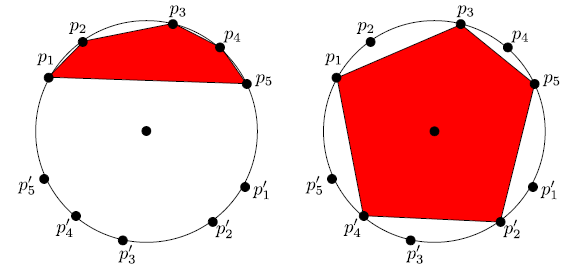
\includegraphics[scale=0.7]{fig1}
%\caption{A thin (left) and a thick (right) antipodal polygon.}
%\end{figure}
\end{frame}

\begin{frame}
\definecolor{ffqqqq}{rgb}{1.,0.,0.}
\begin{figure}
\begin{tikzpicture}[line cap=round,line join=round,>=triangle 45,x=1.0cm,y=1.0cm]
\clip(-5.5,-2.533333333333284) rectangle (10.92,2.353333333333335);
\fill[line width=1.pt,color=ffqqqq,fill=ffqqqq,fill opacity=1.0] (-1.6937799777061364,1.063536265071295) -- (-0.7492357887671589,1.8543585771987179) -- (1.0656265393722786,1.6924656801795013) -- (1.7635692838693833,0.9433045006743214) -- (1.225143330871628,-1.5808301043504873) -- (0.,-2.) -- cycle;
\draw[line width=1.pt] (-1.6937799777061364,1.063536265071295) -- (-0.7492357887671589,1.8543585771987179) -- (1.0656265393722786,1.6924656801795013) -- (1.7635692838693833,0.9433045006743214) -- (1.225143330871628,-1.5808301043504873) -- (0.,-2.) -- cycle;
\draw [line width=1.pt] (0.,0.) circle (2.cm);
\draw [line width=1.pt,color=ffqqqq] (-1.6937799777061364,1.063536265071295)-- (-0.7492357887671589,1.8543585771987179);
\draw [line width=1.pt,color=ffqqqq] (-0.7492357887671589,1.8543585771987179)-- (1.0656265393722786,1.6924656801795013);
\draw [line width=1.pt,color=ffqqqq] (1.0656265393722786,1.6924656801795013)-- (1.7635692838693833,0.9433045006743214);
\draw [line width=1.pt,color=ffqqqq] (1.7635692838693833,0.9433045006743214)-- (1.225143330871628,-1.5808301043504873);
\draw [line width=1.pt,color=ffqqqq] (1.225143330871628,-1.5808301043504873)-- (0.,-2.);
\draw [line width=1.pt,color=ffqqqq] (0.,-2.)-- (-1.6937799777061364,1.063536265071295);
\draw [line width=1.pt] (-1.6937799777061364,1.063536265071295)-- (-0.7492357887671589,1.8543585771987179);
\draw [line width=1.pt] (-0.7492357887671589,1.8543585771987179)-- (1.0656265393722786,1.6924656801795013);
\draw [line width=1.pt] (1.0656265393722786,1.6924656801795013)-- (1.7635692838693833,0.9433045006743214);
\draw [line width=1.pt] (1.7635692838693833,0.9433045006743214)-- (1.225143330871628,-1.5808301043504873);
\draw [line width=1.pt] (1.225143330871628,-1.5808301043504873)-- (0.,-2.);
\draw [line width=1.pt] (0.,-2.)-- (-1.6937799777061364,1.063536265071295);
\draw (-2.1,1.52666666666667) node[anchor=north west] {$p_1$};
\draw (-1.6,2.1) node[anchor=north west] {$p_2$};
\draw (-1.0533333333333343,2.3133333333333366) node[anchor=north west] {$p_3$};
\draw (-0.17333333333333412,2.4866666666666695) node[anchor=north west] {$p_4$};
\draw (1.08,2.1) node[anchor=north west] {$p_5$};
\draw (1.8533333333333328,1.2733333333333368) node[anchor=north west] {$p_6$};
\draw (1.8,-0.86) node[anchor=north west] {$p_1'$};
\draw (1.2,-1.4) node[anchor=north west] {$p_2'$};
\draw (0.6,-1.7) node[anchor=north west] {$p_3'$};
\draw (-0.2,-1.8866666666666623) node[anchor=north west] {$p_4'$};
\draw (-1.4,-1.666666666666624) node[anchor=north west] {$p_5'$};
\draw (-2.4,-0.75) node[anchor=north west] {$p_6'$};
\begin{scriptsize}
\draw [fill=black] (0.,0.) circle (2.0pt);
\draw [fill=black] (0.,2.) circle (2.0pt);
\draw [fill=black] (-0.7492357887671589,1.8543585771987179) circle (2.0pt);
\draw [fill=black] (-1.225143330871628,1.5808301043504873) circle (2.0pt);
\draw [fill=black] (-1.6937799777061364,1.063536265071295) circle (2.0pt);
\draw [fill=black] (1.0656265393722786,1.6924656801795013) circle (2.0pt);
\draw [fill=black] (1.7635692838693833,0.9433045006743214) circle (2.0pt);
\draw [fill=black] (1.6937799777061364,-1.063536265071295) circle (2.0pt);
\draw [fill=black] (1.225143330871628,-1.5808301043504873) circle (2.0pt);
\draw [fill=black] (0.,-2.) circle (2.0pt);
\draw [fill=black] (-1.0656265393722786,-1.6924656801795013) circle (2.0pt);
\draw [fill=black] (-1.7635692838693833,-0.9433045006743214) circle (2.0pt);
\draw [fill=black] (0.7492357887671589,-1.8543585771987179) circle (2.0pt);
\end{scriptsize}
\end{tikzpicture}
\caption{Thick polygon for $n$ even.}
\end{figure}
 
\end{frame}

\begin{frame}
\begin{block}{Remark}
\begin{itemize}
\item<1-> An antipodal polygon $P$ can be neither thick or thin, but it cannot be both at the same time. 
\item<2-> A thin antipodal polygon does not contain the origin and a non-thin polygon always contains it.
\end{itemize}
\end{block}\pause

\only<3->{\begin{block}{Questions}
\begin{itemize}
\item<4-> Does a thick antipodal polygon always have larger area than a thin antipodal polygon?
\item<5-> How efficiently can one compute an antipodal polygon with minimal (maximal)
area?
\item<6-> What can be said about antipodal polygons in higher dimensions?
\end{itemize}
\end{block}}

\end{frame}

\begin{frame}


\frametitle{Where does the inspiration come from?}
\only<2->{
\begin{figure}[h!]
\centering
%
\includegraphics[scale=1.5]{music}
\end{figure}}
\end{frame}

\begin{frame}
\frametitle{Tritones}
A tritone is a musical interval
composed of three whole tones (six semitones).\pause
\vspace{1cm}

\emph{Hey, I'm no music theorist...}


\end{frame}
\begin{frame}
\begin{figure}[h!]
\centering
%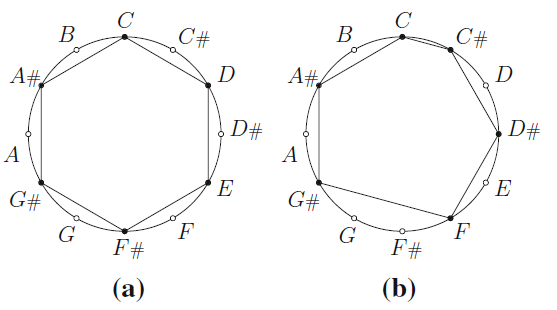
\includegraphics[scale=0.6]{tritone}
\caption{The subsets in a and b represent maximally even scales with and without tritones, respectively}
\end{figure}
\end{frame}


\begin{frame}
\frametitle{Odd rythmic patterns}
\only<1->{A rhythm has the rhythmic oddity property if, when
represented on a circle, it does not contain two onsets.}
\begin{figure}
%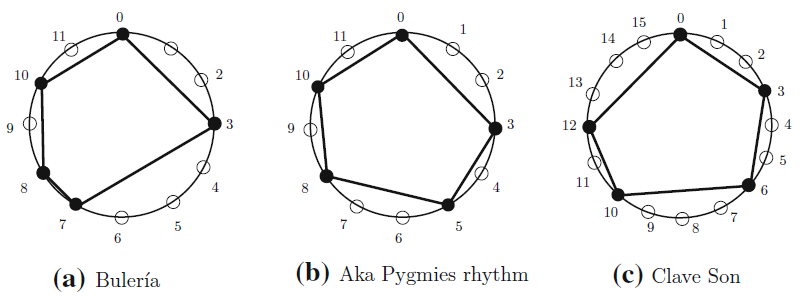
\includegraphics[scale=0.5]{rythm}
\caption{a The bulería rhythm used in Spain, b a rhythm used by the Aka Pygmies of Central Africa, c the
clave son of Cuba}
\end{figure}
\end{frame}

\begin{frame}
\frametitle{Let's get back to work}
\begin{figure}
%
\includegraphics[scale=0.22]{work}
\end{figure}
\end{frame}

\begin{frame}
\frametitle{Results}
\begin{alertblock}{Claim 1}
Given an antipodal point set $S \subset \R^2$, every thin antipodal polygon on $S$ has
less area than any non-thin antipodal polygon on $S$.
\end{alertblock}\pause
\vspace{1cm}

\emph{Is there an exact analogue for thick antipodal polygons?}

\end{frame}

\begin{frame}
\begin{alertblock}{Claim 2}
Given an antipodal point set $S \subset \R^2$, for every non-thick antipodal polygon
on $S$ there exists a thick antipodal polygon on $S$ with larger area.
\end{alertblock}\pause

\begin{figure}
%
\includegraphics[scale=0.6]{close}
\end{figure}
\end{frame}

\begin{frame}
\begin{block}{Remark}
The above claims imply that an antipodal polygon with minimum (resp. maximum)
area is thin (resp. thick). As a consequence, we will show that the extremal
problems for antipodal polygons can be solved in linear time.

\end{block}
\end{frame}


\begin{frame}
\frametitle{Thin Antipodal Polygons}

\begin{itemize}
\item<1-> Assume that the clockwise circular order of $S$ around the origin is $p_1, p_2, \dots , p_n,
p'_1, p'_2,\dots , p'_n$.
\item<2-> For every point $q$ in $S$, let $P_q$ be the thin antipodal polygon that
contains as vertices $q$ and the next $n-1$ clockwise consecutive points of $S$.
\end{itemize}\pause

\begin{figure}
%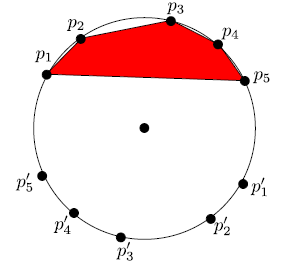
\includegraphics[scale=0.6]{p1}
\caption{$P_{p_1}$}
\end{figure}
\end{frame}

\begin{frame}
\begin{alertblock}{Lemma 1}
For a point $p \in S$ let $l$ be the line containing $p$ and $p'$. Let $\tau$ be the triangle
determined by $p$, and its two neighbors in $S$. Among all triangles that have as vertices
$p$ and one point of $S$ in each of the two half-planes defined by $l$, $\tau$ has strictly the
smallest area.
\end{alertblock}\pause

\begin{proof}
\resizebox{8cm}{5.5cm}{%
\definecolor{qqqqff}{rgb}{0.,0.,1.}
\definecolor{ffqqqq}{rgb}{1.,0.,0.}
\begin{tikzpicture}[line cap=round,line join=round,>=triangle 45,x=1.0cm,y=1.0cm]
\clip(-6.32,-3.8) rectangle (3.8,3.8);
\fill[line width=1.5pt,color=ffqqqq,fill=ffqqqq,fill opacity=0.6000000238418579] (0.,3.) -- (-1.552610542042701,2.566982762843933) -- (2.141426279814696,2.10102201038423) -- cycle;
\fill[line width=2.pt,color=qqqqff,fill=qqqqff,fill opacity=0.07000000029802322] (0.,3.) -- (-2.844054790410907,-0.9546477618162483) -- (2.141426279814696,2.10102201038423) -- cycle;
\draw [line width=1.pt] (0.,0.) circle (3.cm);
\draw [line width=2.pt,color=ffqqqq] (0.,3.)-- (-1.552610542042701,2.566982762843933);
\draw [line width=2.pt,color=ffqqqq] (-1.552610542042701,2.566982762843933)-- (2.141426279814696,2.10102201038423);
\draw [line width=2.pt,color=ffqqqq] (2.141426279814696,2.10102201038423)-- (0.,3.);
\draw [line width=2.pt,color=qqqqff] (0.,3.)-- (-2.844054790410907,-0.9546477618162483);
\draw [line width=2.pt,color=qqqqff] (-2.844054790410907,-0.9546477618162483)-- (2.141426279814696,2.10102201038423);
\draw [line width=2.pt,color=qqqqff] (2.141426279814696,2.10102201038423)-- (0.,3.);
\draw [line width=1.2pt,dash pattern=on 5pt off 5pt] (0.,3.)-- (0.,-3.);
\draw (-0.16,3.6) node[anchor=north west] {\Large{$p$}};
\draw (-0.24,-3) node[anchor=north west] {\Large{$p'$}};
\draw (0.22,0.4) node[anchor=north west] {\Large{$l$}};
\draw (-0.8,2.85) node[anchor=north west] {\large{$\tau$}};
\draw (-1.,1.56) node[anchor=north west] {\large{$\tau'$}};
\draw [color=ffqqqq](0.16,2.3) node[anchor=north west] {\large{$b$}};
\draw [color=qqqqff](0.4,1.1) node[anchor=north west] {\large{$b'$}};
\begin{scriptsize}
\draw [fill=black] (0.,3.) circle (2.5pt);
\draw [fill=black] (-1.552610542042701,2.566982762843933) circle (2.5pt);
\draw [fill=black] (2.141426279814696,2.10102201038423) circle (2.5pt);
\draw [fill=black] (0.,-3.) circle (2.5pt);
\draw [fill=black] (-2.141426279814696,-2.10102201038423) circle (2.5pt);
\draw [fill=black] (1.552610542042701,-2.566982762843933) circle (2.5pt);
\draw [fill=black] (-2.5618223885561213,1.5611105180263856) circle (2.5pt);
\draw [fill=black] (2.844054790410907,0.9546477618162483) circle (2.5pt);
\draw [fill=black] (2.5618223885561213,-1.5611105180263856) circle (2.5pt);
\draw [fill=black] (-2.844054790410907,-0.9546477618162483) circle (2.5pt);
\end{scriptsize}
\end{tikzpicture}
}
\end{proof}
\end{frame}

\begin{frame}
\begin{alertblock}{Lemma 2 (Case $n=3$)}
For $n = 3$, every thin antipodal polygon on $S$ has area strictly less than
that of any non-thin antipodal polygon on $S$.
\end{alertblock}\pause

\begin{proof}
\definecolor{qqqqff}{rgb}{0.,0.,1.}
\definecolor{ffqqqq}{rgb}{1.,0.,0.}
\resizebox{8cm}{5.5cm}{%
\begin{tikzpicture}[line cap=round,line join=round,>=triangle 45,x=1.0cm,y=1.0cm]
\clip(-5.4,-3.7) rectangle (5.,3.76);
\fill[line width=1.5pt,color=ffqqqq,fill=ffqqqq,fill opacity=0.10000000149011612] (-1.9980473079265573,2.2378129848777437) -- (0.,-3.) -- (2.821128677251516,1.0204082449633143) -- cycle;
\fill[line width=2.pt,color=qqqqff,fill=qqqqff,fill opacity=0.10000000149011612] (-2.821128677251516,-1.0204082449633143) -- (0.,3.) -- (1.9980473079265573,-2.2378129848777437) -- cycle;
\draw [line width=1.pt] (0.,0.) circle (3.cm);
\draw [line width=2.pt,color=ffqqqq] (-1.9980473079265573,2.2378129848777437)-- (0.,-3.);
\draw [line width=2.pt,color=ffqqqq] (0.,-3.)-- (2.821128677251516,1.0204082449633143);
\draw [line width=2.pt,color=ffqqqq] (2.821128677251516,1.0204082449633143)-- (-1.9980473079265573,2.2378129848777437);
\draw [line width=2.pt,color=qqqqff] (-2.821128677251516,-1.0204082449633143)-- (0.,3.);
\draw [line width=2.pt,color=qqqqff] (0.,3.)-- (1.9980473079265573,-2.2378129848777437);
\draw [line width=2.pt,color=qqqqff] (1.9980473079265573,-2.2378129848777437)-- (-2.821128677251516,-1.0204082449633143);
\draw (-2.6,2.68) node[anchor=north west] {\large{$p_1$}};
\draw (0.0,3.6) node[anchor=north west] {\large{$p_2$}};
\draw (3.,1.26) node[anchor=north west] {\large{$p_3$}};
\draw (-3.3,-1.08) node[anchor=north west] {\large{$p_3'$}};
\draw (-0.1,-3.) node[anchor=north west] {\large{$p_2'$}};
\draw (2.,-2.2) node[anchor=north west] {\large{$p_1'$}};
\begin{scriptsize}
\draw [fill=black] (0.,3.) circle (2.5pt);
\draw [fill=black] (0.,-3.) circle (2.5pt);
\draw [fill=black] (-1.9980473079265573,2.2378129848777437) circle (2.5pt);
\draw [fill=black] (2.821128677251516,1.0204082449633143) circle (2.5pt);
\draw [fill=black] (1.9980473079265573,-2.2378129848777437) circle (2.5pt);
\draw [fill=black] (-2.821128677251516,-1.0204082449633143) circle (2.5pt);
\end{scriptsize}
\end{tikzpicture}
}
\end{proof}
\end{frame}

\begin{frame}
\begin{alertblock}{Lemma 3 (Case $n=4$)}
For $n = 4$, every thin antipodal polygon on $S$ has area strictly less than
that of any non-thin antipodal polygon on $S$.
\end{alertblock}\pause

\begin{alertblock}{Theorem}
Every thin antipodal polygon on $S$ has less area than any non-thin antipodal
polygon on $S$.
\end{alertblock}\pause
\vspace{0.5cm}

\emph{Idea of the proof}: Induction on $n$ with lemmas 2 and 3 as base cases. Triangulate  a non-thin antipodal poligon $P$ on $S$. Choose wisely and antipodal pair $(p,p')$ that eliminates a thin triangle and use induction on $S\setminus\{p,p'\}$. Then analyse what are the possibilities when adding $p$ or $p'$ to a polygon.
\end{frame}

\section{Thick Antipodal Polygons}
\begin{frame}
\frametitle{Thick Antipodal Polygons}
\begin{block}{Thick Polygon}
Let $S$ be a set of antipodal points in a circle, we say that an antipodal polygon is thick if it has every other point of $S$ along the circle.\\
If the number of points is even we allow only a pair of points of $S$ to be consecutive on the circle.
\end{block}\pause
\vspace{0.5cm}
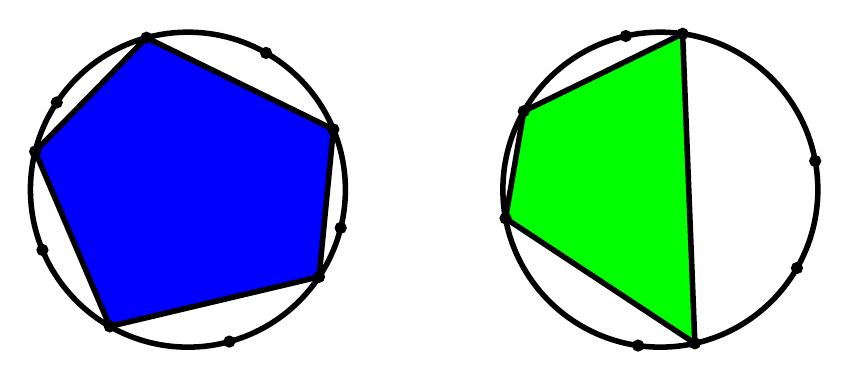
\begin{tikzpicture}
\fill[line width=2pt,fill=blue,fill opacity=1] (-6.940285000290665,-4.514928749927334) -- (-5.526234811584217,-3.0704723575245363) -- (-3.1525157728567357,-4.233969954599134) -- (-3.334444939527694,-6.107215579973068) -- (-5.9922778767136675,-6.736486284248918) -- cycle;
\draw [line width=2pt] (-5,-5) circle (2cm);
\draw [line width=2pt] (-6.940285000290665,-4.514928749927334)-- (-5.526234811584217,-3.0704723575245363);
\draw [line width=2pt] (-5.526234811584217,-3.0704723575245363)-- (-3.1525157728567357,-4.233969954599134);
\draw [line width=2pt] (-3.1525157728567357,-4.233969954599134)-- (-3.334444939527694,-6.107215579973068);
\draw [line width=2pt] (-3.334444939527694,-6.107215579973068)-- (-5.9922778767136675,-6.736486284248918);
\draw [line width=2pt] (-5.9922778767136675,-6.736486284248918)-- (-6.940285000290665,-4.514928749927334);
\begin{scriptsize}
\draw [fill] (-3.059714999709336,-5.485071250072666) circle (2pt);
\draw [fill] (-6.940285000290665,-4.514928749927334) circle (2pt);
\draw [fill] (-6.665555060472307,-3.892784420026933) circle (2pt);
\draw [fill] (-3.334444939527694,-6.107215579973068) circle (2pt);
\draw [fill] (-4.473765188415784,-6.929527642475463) circle (2pt);
\draw [fill] (-5.526234811584217,-3.0704723575245363) circle (2pt);
\draw [fill] (-5.9922778767136675,-6.736486284248918) circle (2pt);
\draw [fill] (-4.007722123286333,-3.263513715751082) circle (2pt);
\draw [fill] (-6.847484227143264,-5.766030045400864) circle (2pt);
\draw [fill] (-3.1525157728567357,-4.233969954599134) circle (2pt);
\end{scriptsize}

\fill[line width=2pt,,fill=green,fill opacity=1] (-0.734733537118563,-4.0046610852598405) -- (-0.9665640099689208,-5.364178520364613) -- (1.4380766846134394,-6.95143250418714) -- (1.2828427124746185,-3.0201010126776677) -- cycle;
\draw [line width=2pt] (1,-5) circle (2cm);
\draw [line width=2pt] (-0.734733537118563,-4.0046610852598405)-- (-0.9665640099689208,-5.364178520364613);
\draw [line width=2pt] (-0.9665640099689208,-5.364178520364613)-- (1.4380766846134394,-6.95143250418714);
\draw [line width=2pt] (1.4380766846134394,-6.95143250418714)-- (1.2828427124746185,-3.0201010126776677);
\draw [line width=2pt] (1.2828427124746185,-3.0201010126776677)-- (-0.734733537118563,-4.0046610852598405);
\begin{scriptsize}
\draw [fill] (2.7347335371185624,-5.9953389147401595) circle (2pt);
\draw [fill] (-0.734733537118563,-4.0046610852598405) circle (2pt);
\draw [fill] (2.96656400996892,-4.635821479635386) circle (2pt);
\draw [fill] (-0.9665640099689208,-5.364178520364613) circle (2pt);
\draw [fill] (1.4380766846134394,-6.95143250418714) circle (2pt);
\draw [fill] (0.5619233153865608,-3.0485674958128595) circle (2pt);
\draw [fill] (0.7171572875253811,-6.979898987322333) circle (2pt);
\draw [fill] (1.2828427124746185,-3.0201010126776677) circle (2pt);
\end{scriptsize}
\end{tikzpicture}
\end{frame}

\begin{frame}
\frametitle{Area increasing operations}
\begin{block}{Flip point}
Given a set of antipodal points $S$ in a circle and an antipodal polygon $P$, we will denote by \emph{flipping} a point $q\in P$ the operation in which we consider a new antipodal polygon $P'$ consisting of the points of $p$ but taking $q'$ instead of $q$.
\end{block}\pause
\begin{alertblock}{Lemma 4.}
If an antipodal polygon $P$ has three consecutive points $p_{1}, p_{2}$ and $p_{3}$ of $S$ as vertices, then flipping $q_{2}$ provides a polygon of larger area.
\end{alertblock}
\end{frame}

\begin{frame}
\frametitle{Three consecutive points}
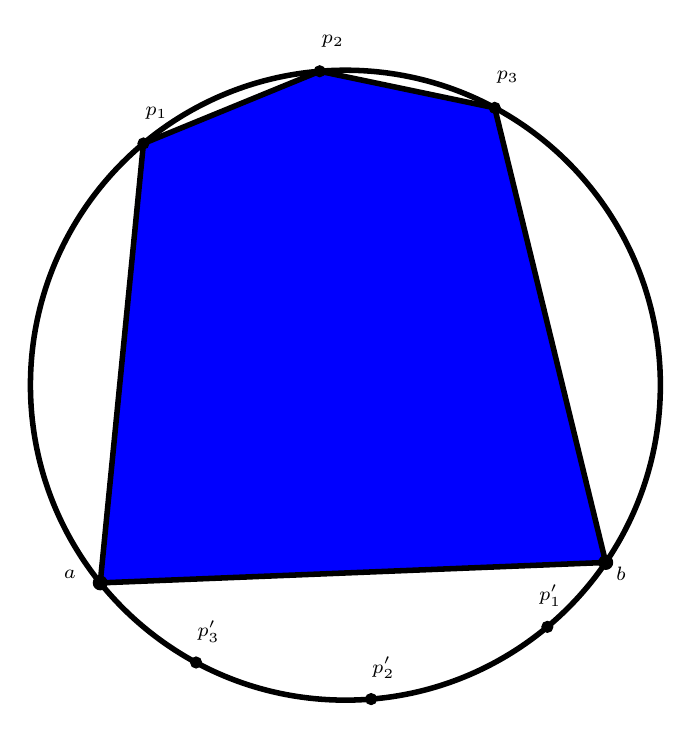
\begin{tikzpicture}
\fill[line width=2pt,fill=blue,fill opacity=1] (-2.564871056390867,3.0694358543693983) -- (-0.3267729577810861,3.98663008492925) -- (1.8963992921400696,3.521884399688701) -- (3.306196213460841,-2.2514587711297755) -- (-3.113652157901318,-2.511009804759126) -- cycle;
\draw [line width=2pt] (0,0) circle (4cm);
\draw [line width=2pt] (-2.564871056390867,3.0694358543693983)-- (-0.3267729577810861,3.98663008492925);
\draw [line width=2pt] (-0.3267729577810861,3.98663008492925)-- (1.8963992921400696,3.521884399688701);
\draw [line width=2pt] (1.8963992921400696,3.521884399688701)-- (3.306196213460841,-2.2514587711297755);
\draw [line width=2pt] (3.306196213460841,-2.2514587711297755)-- (-3.113652157901318,-2.511009804759126);
\draw [line width=2pt] (-3.113652157901318,-2.511009804759126)-- (-2.564871056390867,3.0694358543693983);
\begin{scriptsize}
\draw [fill] (-3.113652157901318,-2.511009804759126) circle (2.5pt);
\draw (-3.5,-2.4) node {$a$};
\draw [fill] (3.306196213460841,-2.2514587711297755) circle (2.5pt);
\draw (3.5,-2.4) node {$b$};
\draw [fill] (2.564871056390867,-3.0694358543693983) circle (2pt);
\draw[] (2.6,-2.67) node {$p_{1}^{\prime}$};
\draw [fill] (-2.564871056390867,3.0694358543693983) circle (2pt);
\draw[] (-2.4,3.45) node {$p_{1}$};
\draw [fill] (0.32677295778108606,-3.9866300849292498) circle (2pt);
\draw[] (0.48,-3.59) node {$p_{2}^{\prime}$};
\draw [fill] (-0.3267729577810861,3.98663008492925) circle (2pt);
\draw[] (-0.16,4.37) node {$p_{2}$};
\draw [fill] (-1.8963992921400696,-3.521884399688701) circle (2pt);
\draw[] (-1.74,-3.13) node {$p_{3}^{\prime}$};
\draw [fill] (1.8963992921400696,3.521884399688701) circle (2pt);
\draw[] (2.06,3.91) node {$p_{3}$};
\end{scriptsize}
\end{tikzpicture}

\end{frame}

\begin{frame}
\frametitle{Three consecutive points}
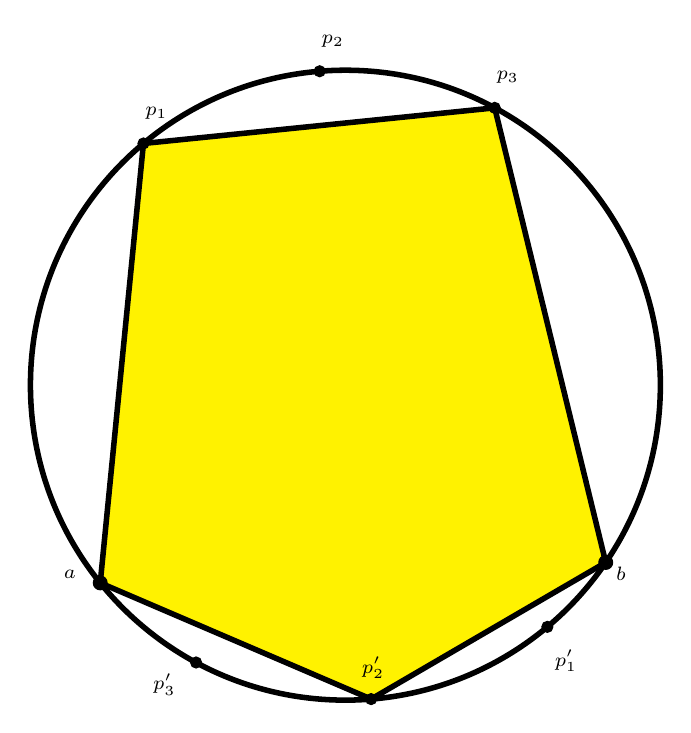
\begin{tikzpicture}
\fill[line width=2pt,fill=yellow,fill opacity=1] (-2.564871056390867,3.0694358543693983) -- (1.8963992921400696,3.521884399688701) -- (3.306196213460841,-2.2514587711297755) -- (0.32677295778108606,-3.9866300849292498) -- (-3.113652157901318,-2.511009804759126) -- cycle;
\draw [line width=2pt] (0,0) circle (4cm);
\draw [line width=2pt] (-2.564871056390867,3.0694358543693983)-- (1.8963992921400696,3.521884399688701);
\draw [line width=2pt] (1.8963992921400696,3.521884399688701)-- (3.306196213460841,-2.2514587711297755);
\draw [line width=2pt] (3.306196213460841,-2.2514587711297755)-- (0.32677295778108606,-3.9866300849292498);
\draw [line width=2pt] (0.32677295778108606,-3.9866300849292498)-- (-3.113652157901318,-2.511009804759126);
\draw [line width=2pt] (-3.113652157901318,-2.511009804759126)-- (-2.564871056390867,3.0694358543693983);
\begin{scriptsize}
\draw [fill] (-3.113652157901318,-2.511009804759126) circle (2.5pt);
\draw (-3.5,-2.4) node {$a$};
\draw [fill] (3.306196213460841,-2.2514587711297755) circle (2.5pt);
\draw (3.5,-2.4) node {$b$};
\draw [fill] (2.564871056390867,-3.0694358543693983) circle (2pt);
\draw[] (2.8,-3.5) node {$p_{1}^{\prime}$};
\draw [fill] (-2.564871056390867,3.0694358543693983) circle (2pt);
\draw[] (-2.4,3.45) node {$p_{1}$};
\draw [fill] (0.32677295778108606,-3.9866300849292498) circle (2pt);
\draw[] (0.35,-3.59) node {$p_{2}^{\prime}$};
\draw [fill] (-0.3267729577810861,3.98663008492925) circle (2pt);
\draw[] (-0.16,4.37) node {$p_{2}$};
\draw [fill] (-1.8963992921400696,-3.521884399688701) circle (2pt);
\draw[] (-2.3,-3.8) node {$p_{3}^{\prime}$};
\draw [fill] (1.8963992921400696,3.521884399688701) circle (2pt);
\draw[] (2.06,3.91) node {$p_{3}$};
\end{scriptsize}
\end{tikzpicture}

\end{frame}

\begin{frame}
\frametitle{Three consecutive points}
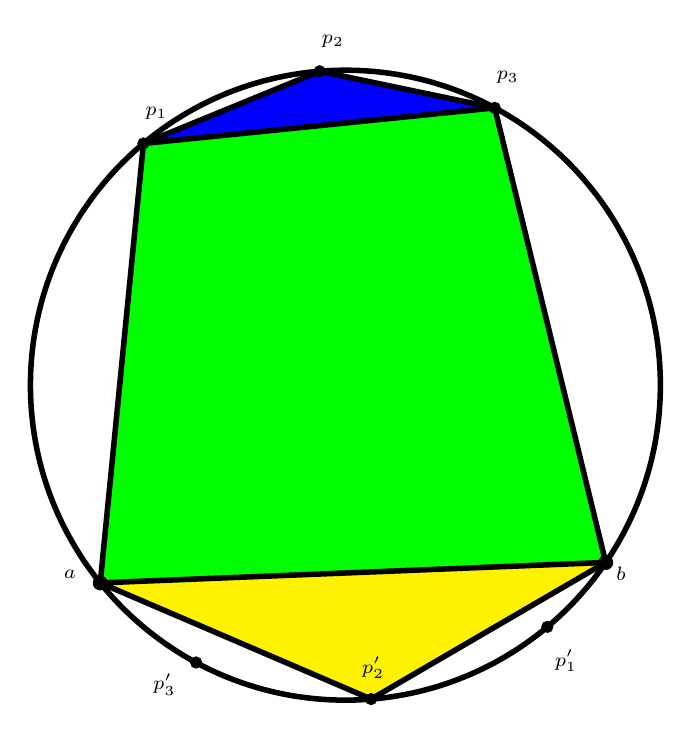
\begin{tikzpicture}
\fill[line width=2pt,fill=yellow,fill opacity=1] (0.32677295778108606,-3.9866300849292498) -- (3.306196213460841,-2.2514587711297755) -- (-3.113652157901318,-2.511009804759126) -- cycle;
\fill[line width=2pt,fill=green,fill opacity=1] (-2.564871056390867,3.0694358543693983) -- (1.8963992921400696,3.521884399688701) -- (3.306196213460841,-2.2514587711297755) -- (-3.113652157901318,-2.511009804759126) -- cycle;
\fill[line width=2pt,fill=blue,fill opacity=1] (-2.564871056390867,3.0694358543693983) -- (1.8963992921400696,3.521884399688701) -- (-0.3267729577810861,3.98663008492925) -- cycle;

\draw [line width=2pt] (0,0) circle (4cm);
\draw [line width=2pt] (3.306196213460841,-2.2514587711297755) -- (-3.113652157901318,-2.511009804759126);
\draw [line width=2pt] (1.8963992921400696,3.521884399688701)-- (-0.3267729577810861,3.98663008492925);
\draw [line width=2pt] (-2.564871056390867,3.0694358543693983)-- (-0.3267729577810861,3.98663008492925);
\draw [line width=2pt] (-2.564871056390867,3.0694358543693983)-- (1.8963992921400696,3.521884399688701);
\draw [line width=2pt] (1.8963992921400696,3.521884399688701)-- (3.306196213460841,-2.2514587711297755);
\draw [line width=2pt] (3.306196213460841,-2.2514587711297755)-- (0.32677295778108606,-3.9866300849292498);
\draw [line width=2pt] (0.32677295778108606,-3.9866300849292498)-- (-3.113652157901318,-2.511009804759126);
\draw [line width=2pt] (-3.113652157901318,-2.511009804759126)-- (-2.564871056390867,3.0694358543693983);
\begin{scriptsize}
\draw [fill] (-3.113652157901318,-2.511009804759126) circle (2.5pt);
\draw (-3.5,-2.4) node {$a$};
\draw [fill] (3.306196213460841,-2.2514587711297755) circle (2.5pt);
\draw (3.5,-2.4) node {$b$};
\draw [fill] (2.564871056390867,-3.0694358543693983) circle (2pt);
\draw[] (2.8,-3.5) node {$p_{1}^{\prime}$};
\draw [fill] (-2.564871056390867,3.0694358543693983) circle (2pt);
\draw[] (-2.4,3.45) node {$p_{1}$};
\draw [fill] (0.32677295778108606,-3.9866300849292498) circle (2pt);
\draw[] (0.35,-3.59) node {$p_{2}^{\prime}$};
\draw [fill] (-0.3267729577810861,3.98663008492925) circle (2pt);
\draw[] (-0.16,4.37) node {$p_{2}$};
\draw [fill] (-1.8963992921400696,-3.521884399688701) circle (2pt);
\draw[] (-2.3,-3.8) node {$p_{3}^{\prime}$};
\draw [fill] (1.8963992921400696,3.521884399688701) circle (2pt);
\draw[] (2.06,3.91) node {$p_{3}$};
\end{scriptsize}
\end{tikzpicture}

\end{frame}

\begin{frame}
\frametitle{Second operation}
\begin{alertblock}{Lemma 5.}
Given a set of antipodal points $S = \{p_{1},\dots,p_{n},p_{1}^{\prime},\dots,p_{n}^{\prime}\}$ in a circle, let $q_{1},\dots,q_{m}$ ($4\leq m\leq n$) be consecutives points of $S$ and let $P$ be an antipodal polygon such that:
\begin{itemize}
\item<2-> $P$ does not contain three consecutive points of $S$.
\item<3-> $P$ contains $q_{1}$ and $q_{2}$.
\item<4-> $P$ either contains $q_{m}$ and $q_{m-1}$ or neither of them.
\item<5-> $P$ contains every other point from $q_{3}$ to $q_{m-1}$.
\end{itemize}

\end{alertblock}

\end{frame}

\begin{frame}
\frametitle{Second operation}
\begin{alertblock}{Lemma 5.}
Given a set of antipodal points $S = \{p_{1},\dots,p_{n},p_{1}^{\prime},\dots,p_{n}^{\prime}\}$ in a circle, let $q_{1},\dots,q_{m}$ ($4\leq m\leq n$) be consecutives points of $S$ and let $P$ be an antipodal polygon such that:
\begin{itemize}
\item $P$ does not contain three consecutive points of $S$.
\item $P$ contains $q_{1}$ and $q_{2}$.
\item $P$ either contains $q_{m}$ and $q_{m-1}$ or neither of them.
\item $P$ contains every other point from $q_{3}$ to $q_{m-1}$.
\end{itemize}
\vspace{0.5cm}
Let $P'$ be the antipodal polygon obtained from $P$ by flipping each $q_{i}$ for $i$ between $2$ and $m-1$, then $P'$ has lager area than $P$.

\end{alertblock}

\end{frame}

\begin{frame}
\frametitle{Second operation}

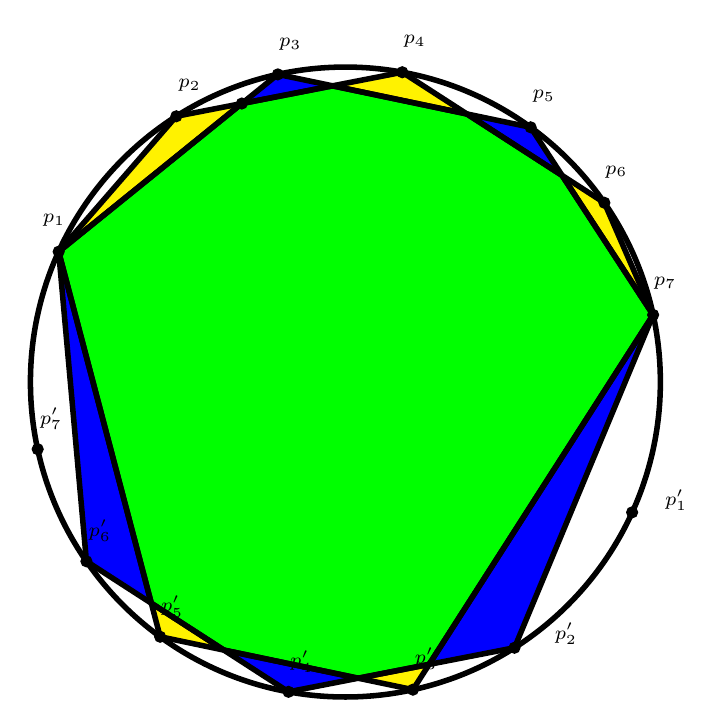
\begin{tikzpicture}
\fill[line width=2pt,fill=yellow,fill opacity=1] (-3.641465909850419,1.6552117772047361) -- (-2.1475019687726373,3.3746459509284294) -- (-1.3151248459184937,3.5369222646648137) -- cycle;
\fill[line width=2pt,fill=blue] (-1.3151248459184937,3.5369222646648137) -- (-0.8576291793704345,3.906977372687535) -- (-0.16292145497981114,3.761550397541616) -- cycle;
\fill[line width=2pt,fill=yellow] (-0.16292145497981114,3.761550397541616) -- (0.7226060813133303,3.9341886649281315) -- (1.5427688824009718,3.404488891541384) -- cycle;
\fill[line width=2pt,fill=blue] (1.5427688824009718,3.404488891541384) -- (2.3526867907001847,3.2349443372127538) -- (2.7518079663665165,2.623634495386156) -- cycle;
\fill[line width=2pt,fill=yellow] (2.7518079663665165,2.623634495386156) -- (3.288768766575114,2.276839915321233) -- (3.908063045639969,0.8526683008669022) -- cycle;
\fill[line width=2pt,fill=blue] (3.908063045639969,0.8526683008669022) -- (2.1475019687726378,-3.3746459509284303) -- (1.0633356844437356,-3.5860098907432385) -- cycle;
\fill[line width=2pt,fill=yellow] (0.8576291793704347,-3.9069773726875354) -- (0.16292145497981128,-3.761550397541616) -- (1.0633356844437356,-3.5860098907432385) -- cycle;
\fill[line width=2pt,fill=blue] (0.16292145497981128,-3.761550397541616) -- (-0.7226060813133303,-3.9341886649281315) -- (-1.5427688824009704,-3.4044888915413845) -- cycle;
\fill[line width=2pt,fill=yellow] (-1.5427688824009704,-3.4044888915413845) -- (-2.352686790700185,-3.2349443372127547) -- (-2.464972496831314,-2.808886353932522) -- cycle;
\fill[line width=2pt,fill=blue] (-2.464972496831314,-2.808886353932522) -- (-3.288768766575114,-2.276839915321233) -- (-3.641465909850419,1.6552117772047361) -- cycle;
\fill[line width=2pt,fill=green] (0.16292145497981128,-3.761550397541616) -- (1.0633356844437356,-3.5860098907432385) -- (3.908063045639969,0.8526683008669022) -- (2.7518079663665165,2.623634495386156) -- (1.5427688824009718,3.404488891541384) -- (-0.16292145497981114,3.761550397541616) -- (-1.3151248459184937,3.5369222646648137) -- (-3.641465909850419,1.6552117772047361) -- (-2.464972496831314,-2.808886353932522) -- (-1.5427688824009704,-3.4044888915413845) -- cycle;
\draw [line width=2pt] (0,0) circle (4cm);
\draw [line width=2pt] (-3.641465909850419,1.6552117772047361)-- (-2.1475019687726373,3.3746459509284294);
\draw [line width=2pt] (-2.1475019687726373,3.3746459509284294)-- (-1.3151248459184937,3.5369222646648137);
\draw [line width=2pt] (-1.3151248459184937,3.5369222646648137)-- (-3.641465909850419,1.6552117772047361);
\draw [line width=2pt] (-1.3151248459184937,3.5369222646648137)-- (-0.8576291793704345,3.906977372687535);
\draw [line width=2pt] (-0.8576291793704345,3.906977372687535)-- (-0.16292145497981114,3.761550397541616);
\draw [line width=2pt] (-0.16292145497981114,3.761550397541616)-- (-1.3151248459184937,3.5369222646648137);
\draw [line width=2pt] (-0.16292145497981114,3.761550397541616)-- (0.7226060813133303,3.9341886649281315);
\draw [line width=2pt] (0.7226060813133303,3.9341886649281315)-- (1.5427688824009718,3.404488891541384);
\draw [line width=2pt] (1.5427688824009718,3.404488891541384)-- (-0.16292145497981114,3.761550397541616);
\draw [line width=2pt] (1.5427688824009718,3.404488891541384)-- (2.3526867907001847,3.2349443372127538);
\draw [line width=2pt] (2.3526867907001847,3.2349443372127538)-- (2.7518079663665165,2.623634495386156);
\draw [line width=2pt] (2.7518079663665165,2.623634495386156)-- (1.5427688824009718,3.404488891541384);
\draw [line width=2pt] (2.7518079663665165,2.623634495386156)-- (3.288768766575114,2.276839915321233);
\draw [line width=2pt] (3.288768766575114,2.276839915321233)-- (3.908063045639969,0.8526683008669022);
\draw [line width=2pt] (3.908063045639969,0.8526683008669022)-- (2.7518079663665165,2.623634495386156);
\draw [line width=2pt] (3.908063045639969,0.8526683008669022)-- (2.1475019687726378,-3.3746459509284303);
\draw [line width=2pt] (2.1475019687726378,-3.3746459509284303)-- (1.0633356844437356,-3.5860098907432385);
\draw [line width=2pt] (1.0633356844437356,-3.5860098907432385)-- (3.908063045639969,0.8526683008669022);
\draw [line width=2pt] (0.8576291793704347,-3.9069773726875354)-- (0.16292145497981128,-3.761550397541616);
\draw [line width=2pt] (0.16292145497981128,-3.761550397541616)-- (1.0633356844437356,-3.5860098907432385);
\draw [line width=2pt] (1.0633356844437356,-3.5860098907432385)-- (0.8576291793704347,-3.9069773726875354);
\draw [line width=2pt] (0.16292145497981128,-3.761550397541616)-- (-0.7226060813133303,-3.9341886649281315);
\draw [line width=2pt] (-0.7226060813133303,-3.9341886649281315)-- (-1.5427688824009704,-3.4044888915413845);
\draw [line width=2pt] (-1.5427688824009704,-3.4044888915413845)-- (0.16292145497981128,-3.761550397541616);
\draw [line width=2pt] (-1.5427688824009704,-3.4044888915413845)-- (-2.352686790700185,-3.2349443372127547);
\draw [line width=2pt] (-2.352686790700185,-3.2349443372127547)-- (-2.464972496831314,-2.808886353932522);
\draw [line width=2pt] (-2.464972496831314,-2.808886353932522)-- (-1.5427688824009704,-3.4044888915413845);
\draw [line width=2pt] (-2.464972496831314,-2.808886353932522)-- (-3.288768766575114,-2.276839915321233);
\draw [line width=2pt] (-3.288768766575114,-2.276839915321233)-- (-3.641465909850419,1.6552117772047361);
\draw [line width=2pt] (-3.641465909850419,1.6552117772047361)-- (-2.464972496831314,-2.808886353932522);
\draw [line width=2pt] (0.16292145497981128,-3.761550397541616)-- (1.0633356844437356,-3.5860098907432385);
\draw [line width=2pt] (1.0633356844437356,-3.5860098907432385)-- (3.908063045639969,0.8526683008669022);
\draw [line width=2pt] (3.908063045639969,0.8526683008669022)-- (2.7518079663665165,2.623634495386156);
\draw [line width=2pt] (2.7518079663665165,2.623634495386156)-- (1.5427688824009718,3.404488891541384);
\draw [line width=2pt] (1.5427688824009718,3.404488891541384)-- (-0.16292145497981114,3.761550397541616);
\draw [line width=2pt] (-0.16292145497981114,3.761550397541616)-- (-1.3151248459184937,3.5369222646648137);
\draw [line width=2pt] (-1.3151248459184937,3.5369222646648137)-- (-3.641465909850419,1.6552117772047361);
\draw [line width=2pt] (-3.641465909850419,1.6552117772047361)-- (-2.464972496831314,-2.808886353932522);
\draw [line width=2pt] (-2.464972496831314,-2.808886353932522)-- (-1.5427688824009704,-3.4044888915413845);
\draw [line width=2pt] (-1.5427688824009704,-3.4044888915413845)-- (0.16292145497981128,-3.761550397541616);
\begin{scriptsize}
\draw [fill] (3.641465909850419,-1.6552117772047361) circle (2pt);
\draw (4.2,-1.5) node {$p_{1}^{\prime}$};
\draw [fill] (-3.641465909850419,1.6552117772047361) circle (2pt);
\draw (-3.7,2.05) node {$p_{1}$};
\draw [fill] (2.1475019687726378,-3.3746459509284303) circle (2pt);
\draw (2.8,-3.2) node {$p_{2}^{\prime}$};
\draw [fill] (-2.1475019687726373,3.3746459509284294) circle (2pt);
\draw (-1.98,3.77) node {$p_{2}$};
\draw [fill] (-0.7226060813133303,-3.9341886649281315) circle (2pt);
\draw (-0.56,-3.55) node {$p_{4}^{\prime}$};
\draw [fill] (0.7226060813133303,3.9341886649281315) circle (2pt);
\draw (0.88,4.33) node {$p_{4}$};
\draw [fill] (-2.352686790700185,-3.2349443372127547) circle (2pt);
\draw (-2.2,-2.85) node {$p_{5}^{\prime}$};
\draw [fill] (2.3526867907001847,3.2349443372127538) circle (2pt);
\draw (2.52,3.63) node {$p_{5}$};
\draw [fill] (-3.908063045639969,-0.8526683008669022) circle (2pt);
\draw (-3.74,-0.47) node {$p_{7}^{\prime}$};
\draw [fill] (3.908063045639969,0.8526683008669022) circle (2pt);
\draw (4.06,1.25) node {$p_{7}$};
\draw [fill] (0.8576291793704347,-3.9069773726875354) circle (2pt);
\draw (1.02,-3.51) node {$p_{3}^{\prime}$};
\draw [fill] (-0.8576291793704345,3.906977372687535) circle (2pt);
\draw (-0.7,4.29) node {$p_{3}$};
\draw [fill] (-3.288768766575114,-2.276839915321233) circle (2pt);
\draw (-3.12,-1.89) node {$p_{6}^{\prime}$};
\draw [fill] (3.288768766575114,2.276839915321233) circle (2pt);
\draw (3.44,2.67) node {$p_{6}$};
\draw [fill] (-1.3151248459184937,3.5369222646648137) circle (2pt);
\end{scriptsize}
\end{tikzpicture}

\end{frame}

\begin{frame}
\frametitle{Second operation}
%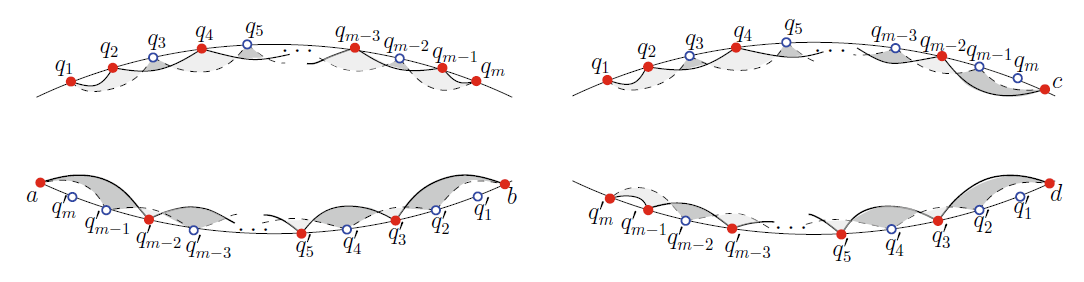
\includegraphics[width=10cm]{polant.png}

\end{frame}

\begin{frame}
\frametitle{Final result}
\begin{alertblock}{Theorem 2.}
Le $S$ be a set of antipodal points in a circle, then, for every non-thick polygon $P$ on $S$, there exists a thick polygon on $S$ with larger area.
\end{alertblock}\pause
\begin{alertblock}{Corollary}
If $S = \{p_{1},\dots,p_{n},p_{1}^{\prime},\dots,p_{n}^{\prime}\}$ and $n$ is odd, then every thick polygon has larger area than a given non-thick polygon.
\end{alertblock}

\end{frame}

\begin{frame}
\frametitle{Counterexample}
Let's see now a counter example for the result with $n = 6$.\pause
\vspace{0.5cm}
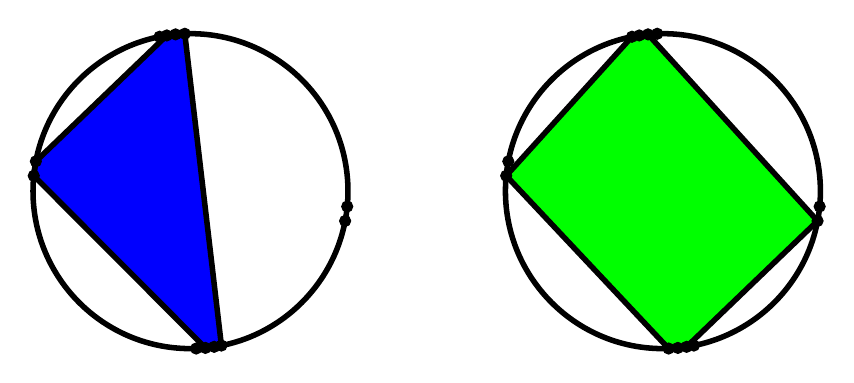
\begin{tikzpicture}
\fill[line width=2pt,fill=blue] (-6.99045705023996,-2.804857151937259) -- (-6.963843933488985,-2.6214276754720034) -- (-5.30041732715371,-1.022691367149321) -- (-5.072310614773505,-1.0013076337287223) -- (-4.606998357000703,-4.961007319874114) -- (-4.810315520976874,-4.990984630382095) -- cycle;
\draw [line width=2pt] (-5,-3) circle (2cm);
\draw [line width=2pt] (-6.99045705023996,-2.804857151937259)-- (-6.963843933488985,-2.6214276754720034);
\draw [line width=2pt] (-6.963843933488985,-2.6214276754720034)-- (-5.30041732715371,-1.022691367149321);
\draw [line width=2pt] (-5.30041732715371,-1.022691367149321)-- (-5.072310614773505,-1.0013076337287223);
\draw [line width=2pt] (-5.072310614773505,-1.0013076337287223)-- (-4.606998357000703,-4.961007319874114);
\draw [line width=2pt] (-4.606998357000703,-4.961007319874114)-- (-4.810315520976874,-4.990984630382095);
\draw [line width=2pt] (-4.810315520976874,-4.990984630382095)-- (-6.99045705023996,-2.804857151937259);
\begin{scriptsize}
\draw [fill] (-3.036156066511018,-3.3785723245279966) circle (2pt);
\draw [fill] (-6.963843933488985,-2.6214276754720034) circle (2pt);
\draw [fill] (-6.99045705023996,-2.804857151937259) circle (2pt);
\draw [fill] (-3.009542949760039,-3.1951428480627406) circle (2pt);
\draw [fill] (-4.606998357000703,-4.961007319874114) circle (2pt);
\draw [fill] (-5.393001642999297,-1.0389926801258866) circle (2pt);
\draw [fill] (-4.699582672846292,-4.97730863285068) circle (2pt);
\draw [fill] (-5.30041732715371,-1.022691367149321) circle (2pt);
\draw [fill] (-4.810315520976874,-4.990984630382095) circle (2pt);
\draw [fill] (-5.189684479023125,-1.0090153696179052) circle (2pt);
\draw [fill] (-4.927689385226497,-4.998692366271277) circle (2pt);
\draw [fill] (-5.072310614773505,-1.0013076337287223) circle (2pt);
\end{scriptsize}
\pause
\fill[line width=2pt,fill=green] (-0.9904570502399599,-2.804857151937259) -- (0.6069983570007027,-1.0389926801258866) -- (0.8103155209768751,-1.0090153696179052) -- (2.963843933488982,-3.3785723245279966) -- (1.300417327153708,-4.97730863285068) -- (1.072310614773503,-4.998692366271277) -- cycle;
\draw [line width=2pt] (1,-3) circle (2cm);
\draw [line width=2pt] (-0.9904570502399599,-2.804857151937259)-- (0.6069983570007027,-1.0389926801258866);
\draw [line width=2pt] (0.6069983570007027,-1.0389926801258866)-- (0.8103155209768751,-1.0090153696179052);
\draw [line width=2pt] (0.8103155209768751,-1.0090153696179052)-- (2.963843933488982,-3.3785723245279966);
\draw [line width=2pt] (2.963843933488982,-3.3785723245279966)-- (1.300417327153708,-4.97730863285068);
\draw [line width=2pt] (1.300417327153708,-4.97730863285068)-- (1.072310614773503,-4.998692366271277);
\draw [line width=2pt] (1.072310614773503,-4.998692366271277)-- (-0.9904570502399599,-2.804857151937259);
\begin{scriptsize}
\draw [fill] (0.6069983570007027,-1.0389926801258866) circle (2pt);
\draw [fill] (-0.9904570502399599,-2.804857151937259) circle (2pt);
\draw [fill] (-0.9638439334889846,-2.6214276754720034) circle (2pt);
\draw [fill] (1.1896844790231258,-4.990984630382095) circle (2pt);
\draw [fill] (1.072310614773503,-4.998692366271277) circle (2pt);
\draw [fill] (1.3930016429992973,-4.961007319874114) circle (2pt);
\draw [fill] (1.300417327153708,-4.97730863285068) circle (2pt);
\draw [fill] (2.963843933488982,-3.3785723245279966) circle (2pt);
\draw [fill] (2.990457050239961,-3.1951428480627406) circle (2pt);
\draw [fill] (0.6995826728462902,-1.022691367149321) circle (2pt);
\draw [fill] (0.8103155209768751,-1.0090153696179052) circle (2pt);
\draw [fill] (0.9276893852264951,-1.0013076337287223) circle (2pt);
\end{scriptsize}
\end{tikzpicture}
\end{frame}

\begin{frame}
\frametitle{Algorithms}
\begin{alertblock}{Minimal area}
There are $\mathcal{O}(n)$ thin polygons, so we can build an algorithm to construct the antipodal polygon which minimizas the area in linear time.
\end{alertblock}\pause
\begin{alertblock}{Maximal area}
There are $\mathcal{O}(n)$ thick polygons, so we can build an algorithm to construct the antipodal polygon which maximized the area in linear time. In the case where $n$ is odd there are only $2$ thick polygons with the same area.
\end{alertblock}
\end{frame}

\begin{frame}
\frametitle{Antipodal polytopes}
We now consider the generalization of the problem, where we have a set $S = \{p_{1},\dots,p_{n},p_{1}^{\prime},\dots,p_{n}^{\prime}\}$ of antipodal points in a $d$-dimensional sphere.\pause
\begin{block}{Thin polytope}
An antipodal polytope is said to be thin if all his vertices lie on the same side of an hyperplane passing through the origin.
\end{block}\pause
\begin{block}{Thick polytope}
An antipodal polytope is said to be thick if for any half-space defined by an hyperplane passing through the origin there are at least $\left \lceil{\frac{n-d}{2}}\right \rceil $ vertices of said polytope contained in the half-space.
\end{block}
\end{frame}

\begin{frame}
\frametitle{Thin antipodal polytopes}
\begin{alertblock}{Can we obtain the same result?}
The previous result does not hold.
\end{alertblock}\pause
\begin{example}
\begin{itemize}
\item<2-> $\epsilon>0$.
\item<3-> $\delta = \sqrt{1-2\epsilon^{2}}$.
\item<4-> $v_{1} = (0,0,1);v_{2}= (\delta,\epsilon,\epsilon);v_{3}= (-\delta,\epsilon,\epsilon);v_{4}= (\epsilon,\delta,\epsilon);v_{5}= (\epsilon,-\delta,\epsilon)$.
\item<5-> $S_{1} = \{v_{1},\dots,v_{5}\}$ whose volume converges to $2/3$ when $\epsilon\to 0$.
\item<6-> $S_{2} = \{v_{1}^{\prime},v_{2}^{\prime},v_{3},v_{4},v_{5}\}$ whose volume converges to $1/3$ when $\epsilon\to 0$.
\end{itemize}
\end{example}
\end{frame}

\begin{frame}
\begin{figure}
%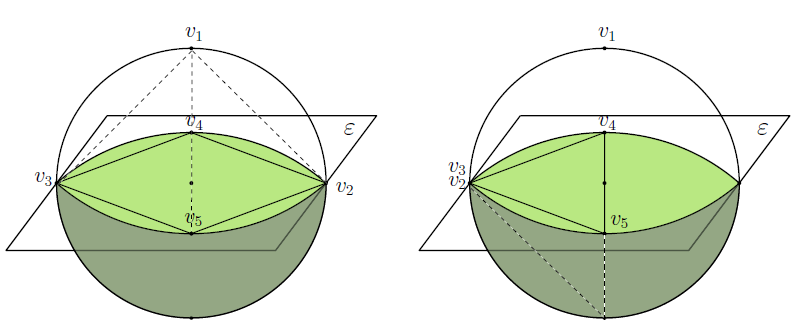
\includegraphics[scale=0.5]{esfera}
\end{figure}
\end{frame}

\begin{frame}
\frametitle{Thick antipodal polytopes}
Must there exist a thick antipodal polytope for any given set of antipodal points?
\begin{alertblock}{Lemma.}
If $n\geq d$, using Gale's Lemma we can construct a thick antipodal polytope from a given set of points $S= \{p_{1},\dots,p_{n},p_{1}^{\prime},\dots,p_{n}^{\prime}\}$.
\end{alertblock}

\end{frame}

\section{Open Problem}
\begin{frame}
\frametitle{Open Problem}
Let us assume that we are given a circular lattice with an antipodal set of $2n$ points
(evenly spaced) and we would like to compute an extremal antipodal $k$-polygon with
$k < n$ vertices.

\definecolor{zzttqq}{rgb}{0.6,0.2,0.}
\begin{figure}
\begin{tikzpicture}[line cap=round,line join=round,>=triangle 45,x=1.0cm,y=1.0cm]
\clip(-5,-2.066666666666644) rectangle (9.086666666666668,2.5);
\fill[line width=2.pt,color=zzttqq,fill=zzttqq,fill opacity=0.10000000149011612] (-1.7557911458287687,0.9577042613611466) -- (0.,2.) -- (1.0229677195353655,1.7185857688194133) -- (1.755791145828769,0.9577042613611464) -- (2.,0.) -- cycle;
\draw [line width=1.2pt] (0.,0.) circle (2.cm);
\draw [line width=2.pt,color=zzttqq] (-1.7557911458287687,0.9577042613611466)-- (0.,2.);
\draw [line width=2.pt,color=zzttqq] (0.,2.)-- (1.0229677195353655,1.7185857688194133);
\draw [line width=2.pt,color=zzttqq] (1.0229677195353655,1.7185857688194133)-- (1.755791145828769,0.9577042613611464);
\draw [line width=2.pt,color=zzttqq] (1.755791145828769,0.9577042613611464)-- (2.,0.);
\draw [line width=2.pt,color=zzttqq] (2.,0.)-- (-1.7557911458287687,0.9577042613611466);
\begin{scriptsize}
\draw [fill=black] (0.,0.) circle (1.5pt);
\draw [fill=black] (0.,2.) circle (2.0pt);
\draw [fill=black] (-1.0229677195353652,1.7185857688194135) circle (2.0pt);
\draw [fill=black] (-1.7557911458287687,0.9577042613611466) circle (2.0pt);
\draw [fill=black] (-2.,0.) circle (2.0pt);
\draw [fill=black] (0.,-2.) circle (2.0pt);
\draw [fill=black] (1.0229677195353652,-1.7185857688194135) circle (2.0pt);
\draw [fill=black] (1.7557911458287687,-0.9577042613611466) circle (2.0pt);
\draw [fill=black] (2.,0.) circle (2.0pt);
\draw [fill=black] (1.0229677195353655,1.7185857688194133) circle (2.0pt);
\draw [fill=black] (1.755791145828769,0.9577042613611464) circle (2.0pt);
\draw [fill=black] (-1.755791145828769,-0.9577042613611464) circle (2.0pt);
\draw [fill=black] (-1.0229677195353655,-1.7185857688194133) circle (2.0pt);
\end{scriptsize}
\end{tikzpicture}
\caption{$n=6$, $k=5$.}
\end{figure}
\end{frame}

\begin{frame}
Finding the extremal antipodal $(n-1)$-polygon, called $(2n, n-1)$-problem for short, can be easily
reduced to solve $\mathcal{O}(n)$ times the $(2(n - 1), n - 1)$-problem: \pause
\vspace{0.5cm}

In the $(2n, n - 1)$-problem an antipodal pair is not selected and can thus be removed
from the input. This approach gives a simple $\mathcal{O}(n^{n-k+1})$ time algorithm for solving
the general $(2n, k)$-problem.\pause
\vspace{0.5cm}

\begin{alertblock}{Open Problem}
Can the $(2n,k)$-problem be solved in $\mathcal{O}(n^k)$ time?
\end{alertblock}

\end{frame}

\begin{frame}
\begin{figure}
%
\includegraphics[scale=1]{folks}
\end{figure}
\end{frame}



\end{document}
